\section{Antenna Design 2 -- Triangle-Feed Antenna}
\fixme{Insert results for the talk/play/read mode and SAR results.}
\begin{figure}[htbp]
    \centering
    \begin{subfigure}[b]{0.24\linewidth}
        \centering
        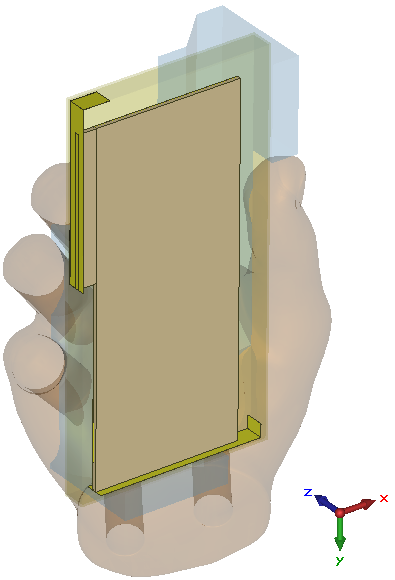
\includegraphics[width=\linewidth,height=4cm,keepaspectratio]{img/tech_sol/trianglefeed/read_mode/3d.PNG}
        \caption{Read mode.}
    \end{subfigure}
    \begin{subfigure}[b]{0.24\linewidth}
        \centering
        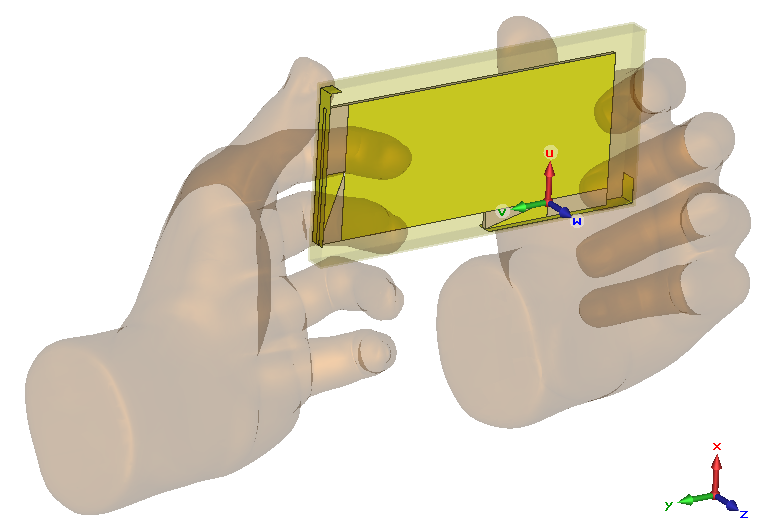
\includegraphics[width=\linewidth,height=4cm,keepaspectratio]{img/tech_sol/trianglefeed/play_mode/3d.PNG}
        \caption{Play mode.}
    \end{subfigure}
    \begin{subfigure}[b]{0.24\linewidth}
        \centering
        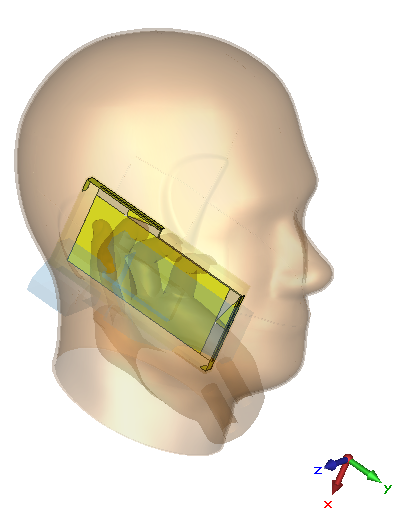
\includegraphics[width=\linewidth,height=4cm,keepaspectratio]{img/tech_sol/trianglefeed/talk_mode/3d.PNG}
        \caption{Talk mode.}
    \end{subfigure}
    \begin{subfigure}[b]{0.24\linewidth}
        \centering
        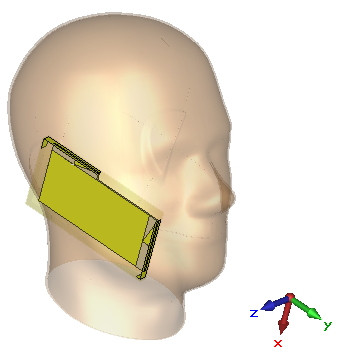
\includegraphics[width=\linewidth,height=4cm,keepaspectratio]{img/tech_sol/trianglefeed/sar/3d.PNG}
        \caption{SAR.}
    \end{subfigure}
    \caption{Antenna position for each user effect simulation.}
    \label{fig:triang_positions}
\end{figure}

\subsection{Read Mode}

\begin{figure}[htbp]
    \centering
    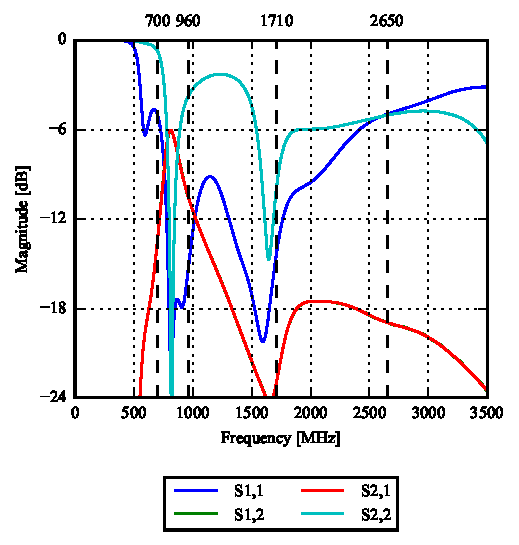
\includegraphics{img/tech_sol/trianglefeed/read_mode/sparams.pdf}
    \caption{Triangular feed antenna in read mode. S-parameters with both tuning capacitors fixed at \SI{0.3}{pF}.}
    \label{fig:triang_sparam_read}
\end{figure}

\begin{figure}[htbp]
   \begin{subfigure}[b]{0.49\linewidth}
        \centering
        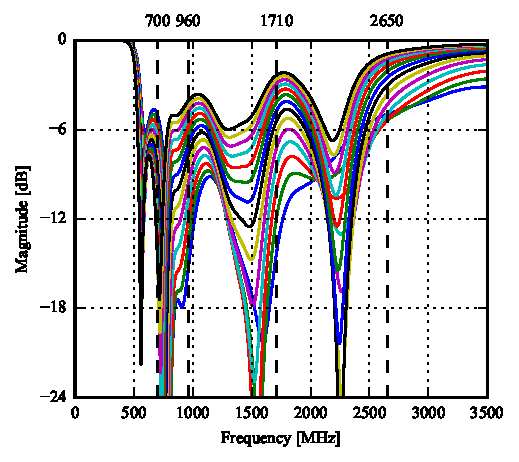
\includegraphics{img/tech_sol/trianglefeed/read_mode/Csh1s11.pdf}
        \caption{$S_{11}$, sweeping $C_1$ and fixing $C_2$.}
    \end{subfigure}
    \hfill
    \begin{subfigure}[b]{0.49\linewidth}
        \centering
        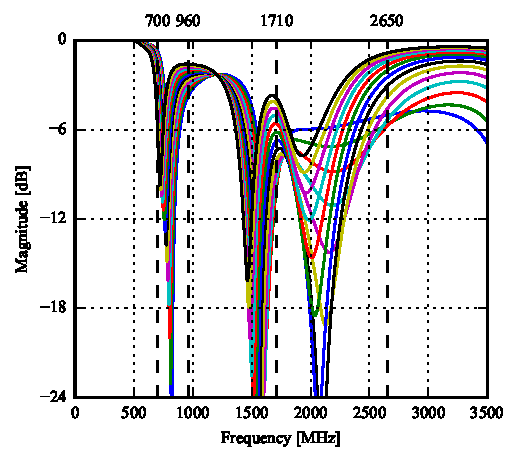
\includegraphics{img/tech_sol/trianglefeed/read_mode/Csh2s22.pdf}
        \caption{$S_{22}$, sweeping $C_1$ and fixing $C_2$.}
    \end{subfigure}
    \\
    \begin{subfigure}[b]{0.49\linewidth}
        \centering
        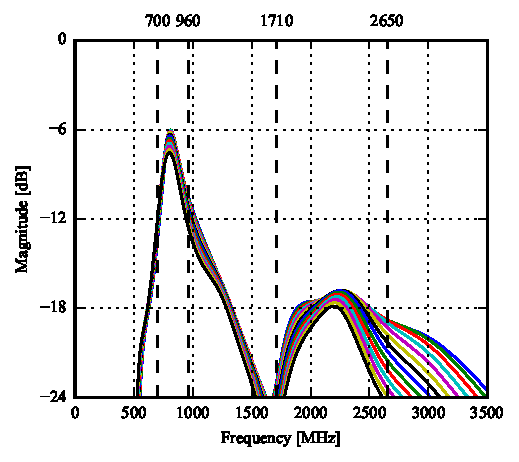
\includegraphics{img/tech_sol/trianglefeed/read_mode/Csh1s21.pdf}
        \caption{$S_{21}$, sweeping $C_1$ and fixing $C_2$.}
    \end{subfigure}
    \hfill
    \begin{subfigure}[b]{0.49\linewidth}
        \centering
        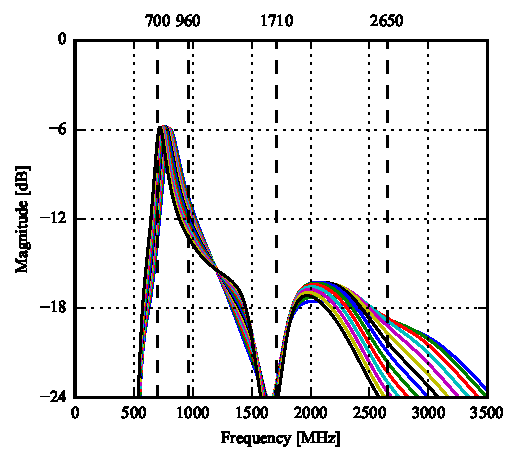
\includegraphics{img/tech_sol/trianglefeed/read_mode/Csh2s21.pdf}
        \caption{$S_{21}$, sweeping $C_2$ and fixing $C_1$.}
    \end{subfigure}
    \caption{Triangle feed antenna in read mode. Parameter sweep for tuning the shunt capacitor of each antenna, $C_1$ and $C_2$ for port 1 and 2, respectively. Port 1 is the top antenna and port 2 is the side antenna.}
    \label{fig:tiang_sparam_sweep_read}
\end{figure}


\subsection{Play Mode}

\begin{figure}[htbp]
    \centering
    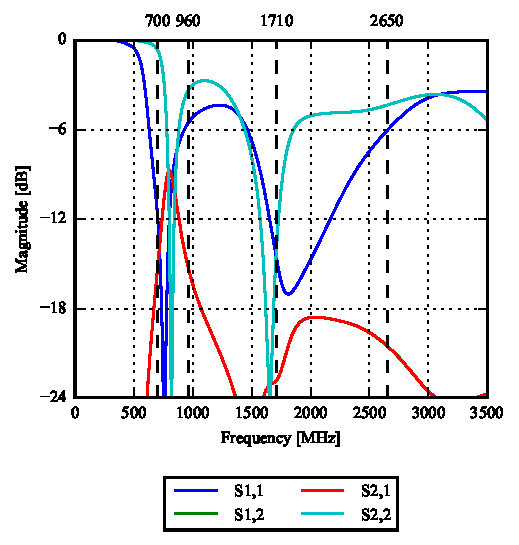
\includegraphics{img/tech_sol/trianglefeed/play_mode/sparams.pdf}
    \caption{Triangular feed antenna in play mode. S-parameters with both tuning capacitors fixed at \SI{0.3}{pF}.}
    \label{fig:triang_sparam_play}
\end{figure}

\begin{figure}[htbp]
   \begin{subfigure}[b]{0.49\linewidth}
        \centering
        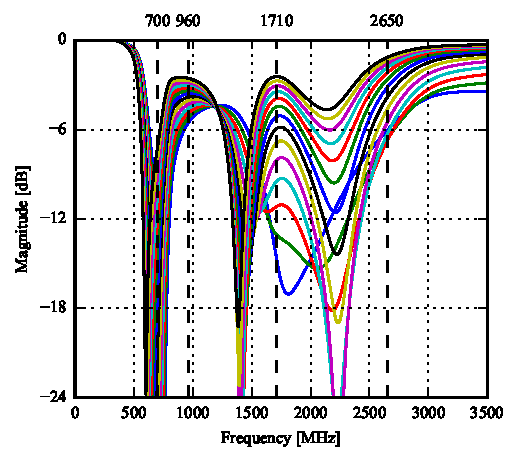
\includegraphics{img/tech_sol/trianglefeed/play_mode/Csh1s11.pdf}
        \caption{$S_{11}$, sweeping $C_1$ and fixing $C_2$.}
    \end{subfigure}
    \hfill
    \begin{subfigure}[b]{0.49\linewidth}
        \centering
        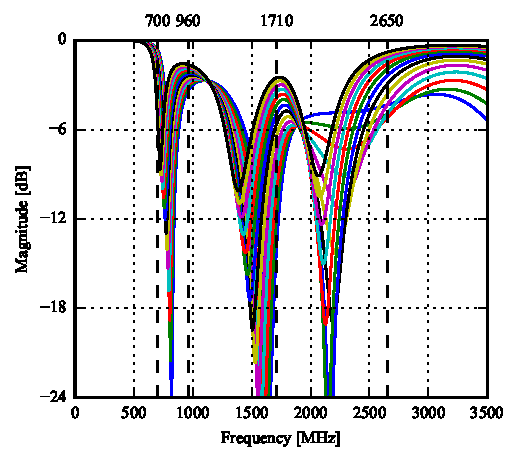
\includegraphics{img/tech_sol/trianglefeed/play_mode/Csh2s22.pdf}
        \caption{$S_{22}$, sweeping $C_1$ and fixing $C_2$.}
    \end{subfigure}
    \\
    \begin{subfigure}[b]{0.49\linewidth}
        \centering
        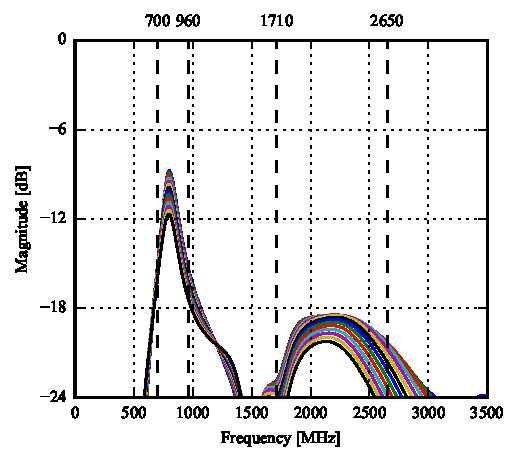
\includegraphics{img/tech_sol/trianglefeed/play_mode/Csh1s21.pdf}
        \caption{$S_{21}$, sweeping $C_1$ and fixing $C_2$.}
    \end{subfigure}
    \hfill
    \begin{subfigure}[b]{0.49\linewidth}
        \centering
        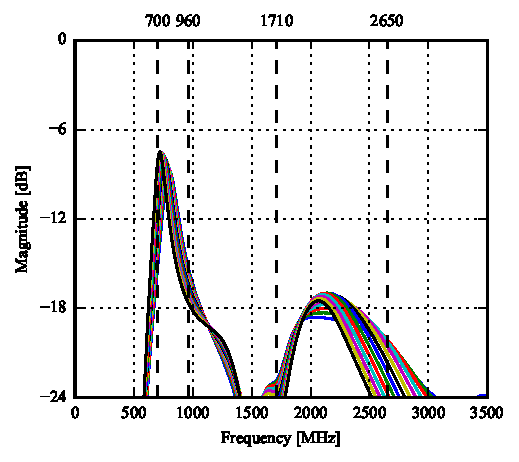
\includegraphics{img/tech_sol/trianglefeed/play_mode/Csh2s21.pdf}
        \caption{$S_{21}$, sweeping $C_2$ and fixing $C_1$.}
    \end{subfigure}
    \caption{Triangle feed antenna in play mode. Parameter sweep for tuning the shunt capacitor of each antenna, $C_1$ and $C_2$ for port 1 and 2, respectively. Port 1 is the top antenna and port 2 is the side antenna.}
    \label{fig:tiang_sparam_sweep_play}
\end{figure}

\subsection{Talk Mode}

\begin{figure}[htbp]
    \centering
    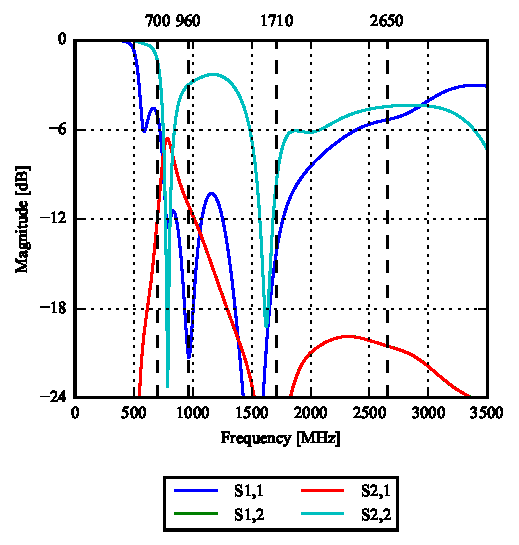
\includegraphics{img/tech_sol/trianglefeed/talk_mode/sparams.pdf}
    \caption{Triangular feed antenna in talk mode. S-parameters with both tuning capacitors fixed at \SI{0.3}{pF}.}
    \label{fig:triang_sparam_talk}
\end{figure}

\begin{figure}[htbp]
   \begin{subfigure}[b]{0.49\linewidth}
        \centering
        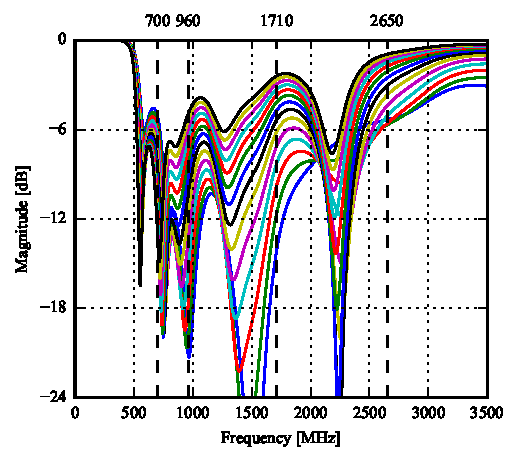
\includegraphics{img/tech_sol/trianglefeed/talk_mode/Csh1s11.pdf}
        \caption{$S_{11}$, sweeping $C_1$ and fixing $C_2$.}
    \end{subfigure}
    \hfill
    \begin{subfigure}[b]{0.49\linewidth}
        \centering
        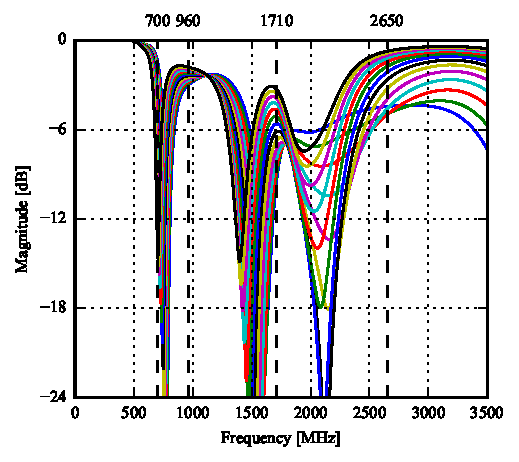
\includegraphics{img/tech_sol/trianglefeed/talk_mode/Csh2s22.pdf}
        \caption{$S_{22}$, sweeping $C_1$ and fixing $C_2$.}
    \end{subfigure}
    \\
    \begin{subfigure}[b]{0.49\linewidth}
        \centering
        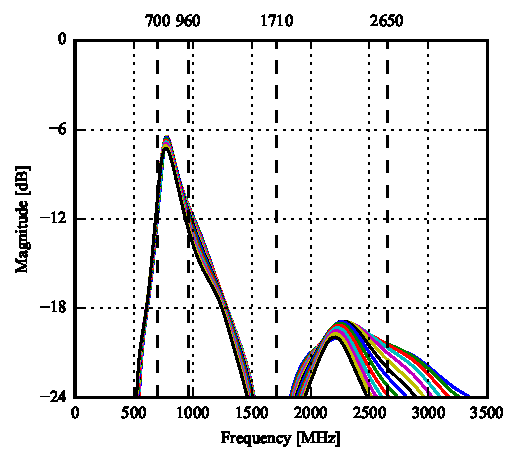
\includegraphics{img/tech_sol/trianglefeed/talk_mode/Csh1s21.pdf}
        \caption{$S_{21}$, sweeping $C_1$ and fixing $C_2$.}
    \end{subfigure}
    \hfill
    \begin{subfigure}[b]{0.49\linewidth}
        \centering
        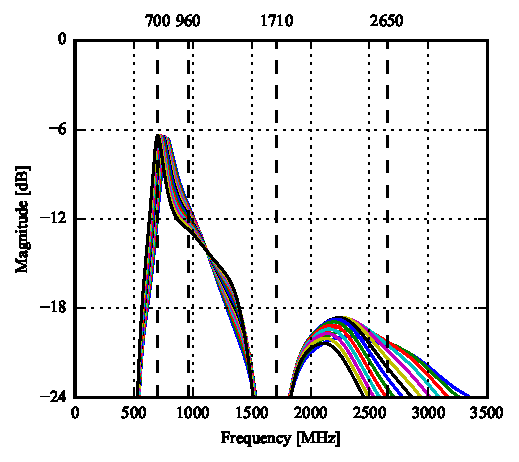
\includegraphics{img/tech_sol/trianglefeed/talk_mode/Csh2s21.pdf}
        \caption{$S_{21}$, sweeping $C_2$ and fixing $C_1$.}
    \end{subfigure}
    \caption{Triangle feed antenna in talk mode. Parameter sweep for tuning the shunt capacitor of each antenna, $C_1$ and $C_2$ for port 1 and 2, respectively. Port 1 is the top antenna and port 2 is the side antenna.}
    \label{fig:tiang_sparam_sweep_talk}
\end{figure}

\subsection{SAR}


